\thispagestyle{empty}
\null
\vfill
\begin{center}

   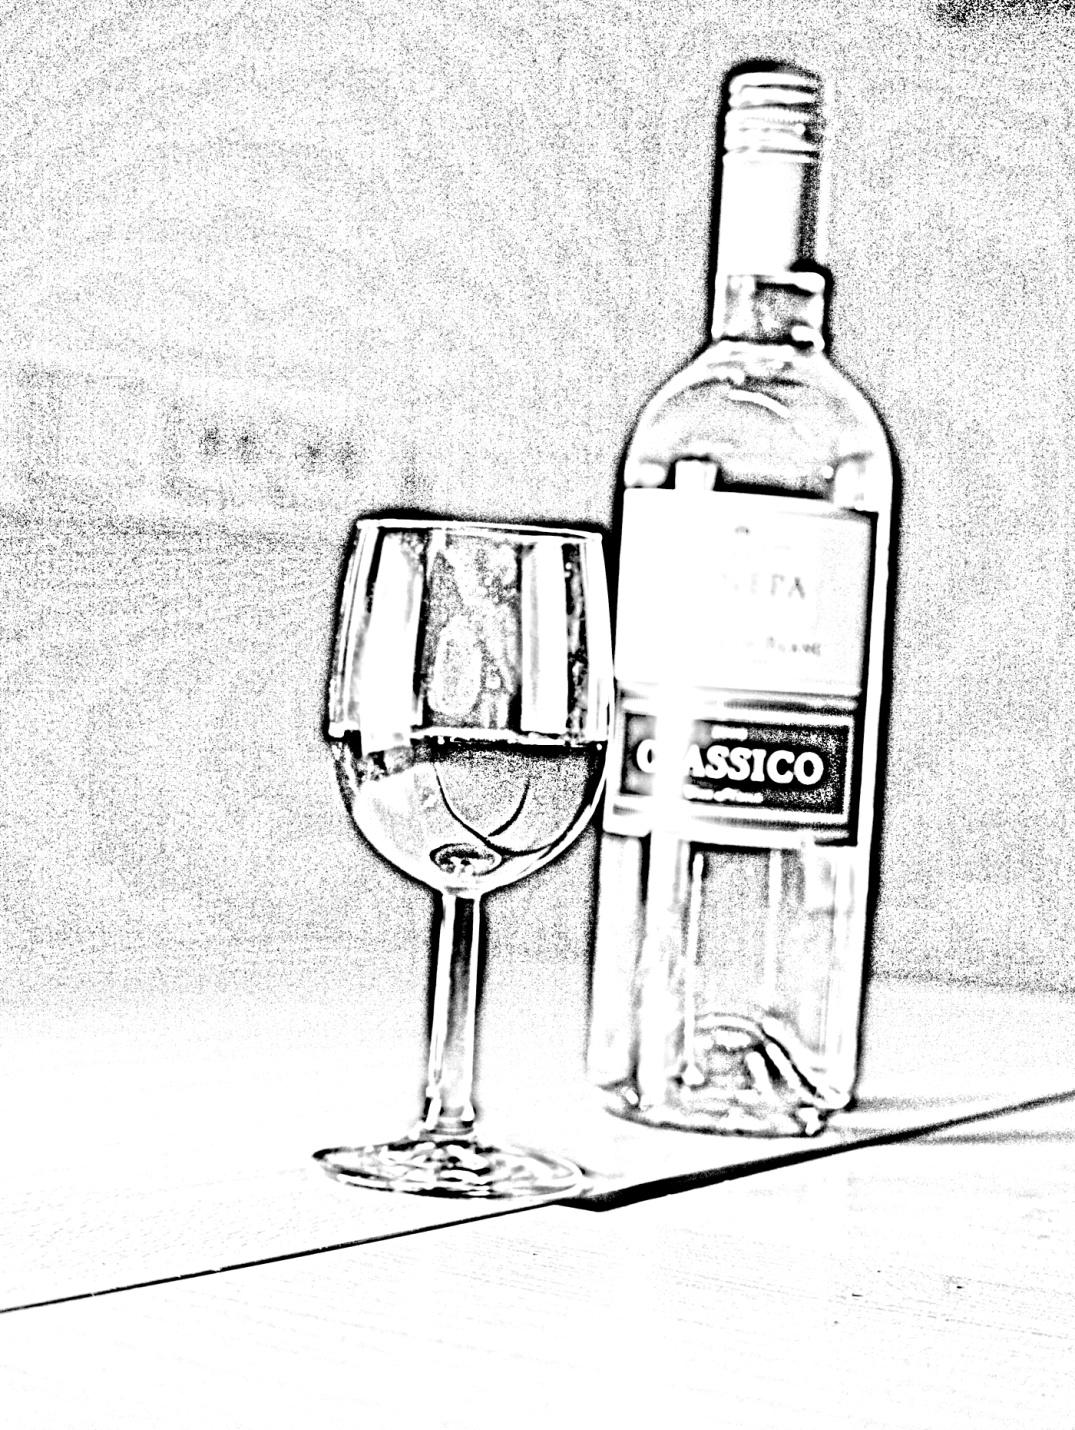
\includegraphics[width=0.8\textwidth]{res/vinvisor.jpg}
   \section{Vinvisor}

\end{center}
\vfill
\newpage


\subsection{Bordeaux, Bordeaux}
\textit{Mel: I sommarens soliga dagar}\\
\index[alfa]{Bordeaux, Bordeaux}
\index[anfa]{Jag minns än idag hur min fader...}
\begin{parse lines}[\noindent]{#1\\}

Jag minns än idag hur min fader
kom hem ifrån staden så glader
och rada upp flaskor i rader
och sade nöjd som så:
``Bordeaux, Bordeaux!''

Han drack ett glas, kom i extas,
och sedan blev det stort kalas.
Och vi små glin, ja vi drack vin
som första klassens fyllesvin.
Och vi dansade runt där på borden
och skrek så vi blev blå:
``Bordeaux, Bordeaux!''
\end{parse lines}


\subsection{Ismaskinen}
\textit{Mel: Nu så kommer julen, ur Karl-Bertil Johnssons julafton}\\
\textit{Lundakarnevalen 2002}\\
\index[alfa]{Ismaskinen}
\index[anfa]{Läpparna blir lila...}
\begin{parse lines}[\noindent]{#1\\}

Läpparna blir lila
när man dricker vin,
och om man har huvet
i en ismaskin!
\end{parse lines}


\subsection{Feta fransyskor}
\textit{Mel: Militärmarsch av Schubert}\\
\textit{K-sektionen Sångarstriden 1985}\\
\index[alfa]{Feta fransyskor}
\index[anfa]{Feta fransyskor som svettas om fötterna...}
\begin{parse lines}[\noindent]{#1\\}

Feta fransyskor som svettas om fötterna,
de trampar druvor
som sedan ska jäsas till vin.
Transpirationen viktig é,
ty den ge
fin bouquet.
Vårtor och svampar följer me'
men vad gör väl de'?

För vi vill ha vin,
vill ha vin,
vill ha mera vin,
även om följderna blir
att vi må lida pin.
Flaskan och glaset gått i sin.
Hit med vin, mera vin!
Tror ni att vi är fyllesvin?
Ja! Fast större!
\end{parse lines}
\vfill
\noindent\textit{Att man i slutet sjunger ``Ja! Fast större!'' var inte menat från
  början, utan det var menat att tryckeriet skulle trycka ``Ja!'' med större
  bokstäver.}



\subsection{Korkskruvens visa}
\textit{Mel: Nu har vi ljus}\\
\index[alfa]{Korkskruvens visa}
\index[anfa]{Nu har vi rus här i vårt hus...}
\begin{parse lines}[\noindent]{#1\\}

Nu har vi rus här i vårt hus
Korken är borta hopptralalala
Doften är ljuv, jag är en skruv,
jag är en skruv.

Jag kan inte öppna bag-in-boxen,
jag kan inte öppna bag-in-boxen

Lalalala lalalala lalalalala lala
\end{parse lines}


\subsection{Vinvännernas visa}
\textit{Mel: Imse vimse spindel}\\
\index[alfa]{Vinvännernas visa}
\index[anfa]{Åsnan dricker vatten, det gör inte vi...}
\begin{parse lines}[\noindent]{#1\\}

Åsnan dricker vatten, det gör inte vi.
Vi dricker bara sådant folk har trampat i.
Kamelen uti öknen söker en oas,
det gör inte vi, vi har vin i våra glas.

Imse vimse blir jag utav lite vin.
Kliver upp på stolen, och blir piggelin.
Trillar under bordet, sussar en minut.
Vaknar av att vinet nästan tagit slut.
\end{parse lines}


\subsection{Magnumflaskan Åkesson}
\textit{Mel: Teddybjörnen Fredriksson}\\
\index[alfa]{Magnumflaskan Åkesson}
\index[anfa]{För längesen, när jag fyllde 15 år...}
\begin{parse lines}[\noindent]{#1\\}

För längesen, när jag fyllde 15 år
fick jag en flaska av min mor.
Hon sa ``Mitt barn, dela den med vännerna.
För den är faktiskt ganska stor.''

Magnumflaskan Åkesson,
du var så stor och tung.
Jag gick runt med dig i hand,
och i Dalby var jag kung.

Magnumflaskan Åkesson,
din kork försvann i skyn.
Men jag drack dig bara själv.
Och kräktes i hela byn.
\end{parse lines}

\newpage
\subsection{Sprittillverkarvisan}
\textit{Mel: Mössens julafton}\\
\index[alfa]{Sprittillverkarvisan}
\index[anfa]{För väldigt många år sen plantera man i rad...}
\begin{parse lines}[\noindent]{#1\\}

För väldigt många år sen plantera man i rad
små rankor för att göra drycker så att man blev glad.
En druva skulle odlas och efter något år
bli plockad, trampad, tappad och sen fin Bordeaux.
Konstiga processer tog sin fart,
men det tog alltför många år för vinet att bli klart.
Ty idag med socker, jäst och vann
på någon dag man gör sin alkohol i spann.
\end{parse lines}
